%!TEX root = ../template.tex
%%%%%%%%%%%%%%%%%%%%%%%%%%%%%%%%%%%%%%%%%%%%%%%%%%%%%%%%%%%%%%%%%%%
%% chapter1.tex
%% NOVA thesis document file
%%
%% Chapter with introduction
%%%%%%%%%%%%%%%%%%%%%%%%%%%%%%%%%%%%%%%%%%%%%%%%%%%%%%%%%%%%%%%%%%%

\typeout{NT FILE chapter1.tex}%

\chapter{Introduction}
\label{cha:introduction}

\section{Motivation \& Problem Statement}
\label{sec:motivation+problem-statement}
\subsection{Breast Cancer - A Global Health Challenge}

\gls{BC} is currently one of the biggest public health challenges worldwide. In 
2022, more than $2.3$ million new cases of \gls{BC} were diagnosed, resulting in
around $665,\!000$ global deaths \textcite{bcaData2024_bray}. Other studies 
estimate that \gls{BC} will continue to not only bethe most commonly diagnosed 
cancer but also to increase in incidence, with projections indicating that by 
2040, the number of deaths will almost double and the number of new cases will 
be around $3.2$ million \textcite{bca_data_Arnold2022Current}. These figures 
underline the high incidence and mortality associated with the disease, 
highlighting the ongoing need to develop more effective strategies for 
its diagnosis and treatment.

\begin{figure}[h!]
  \centering
  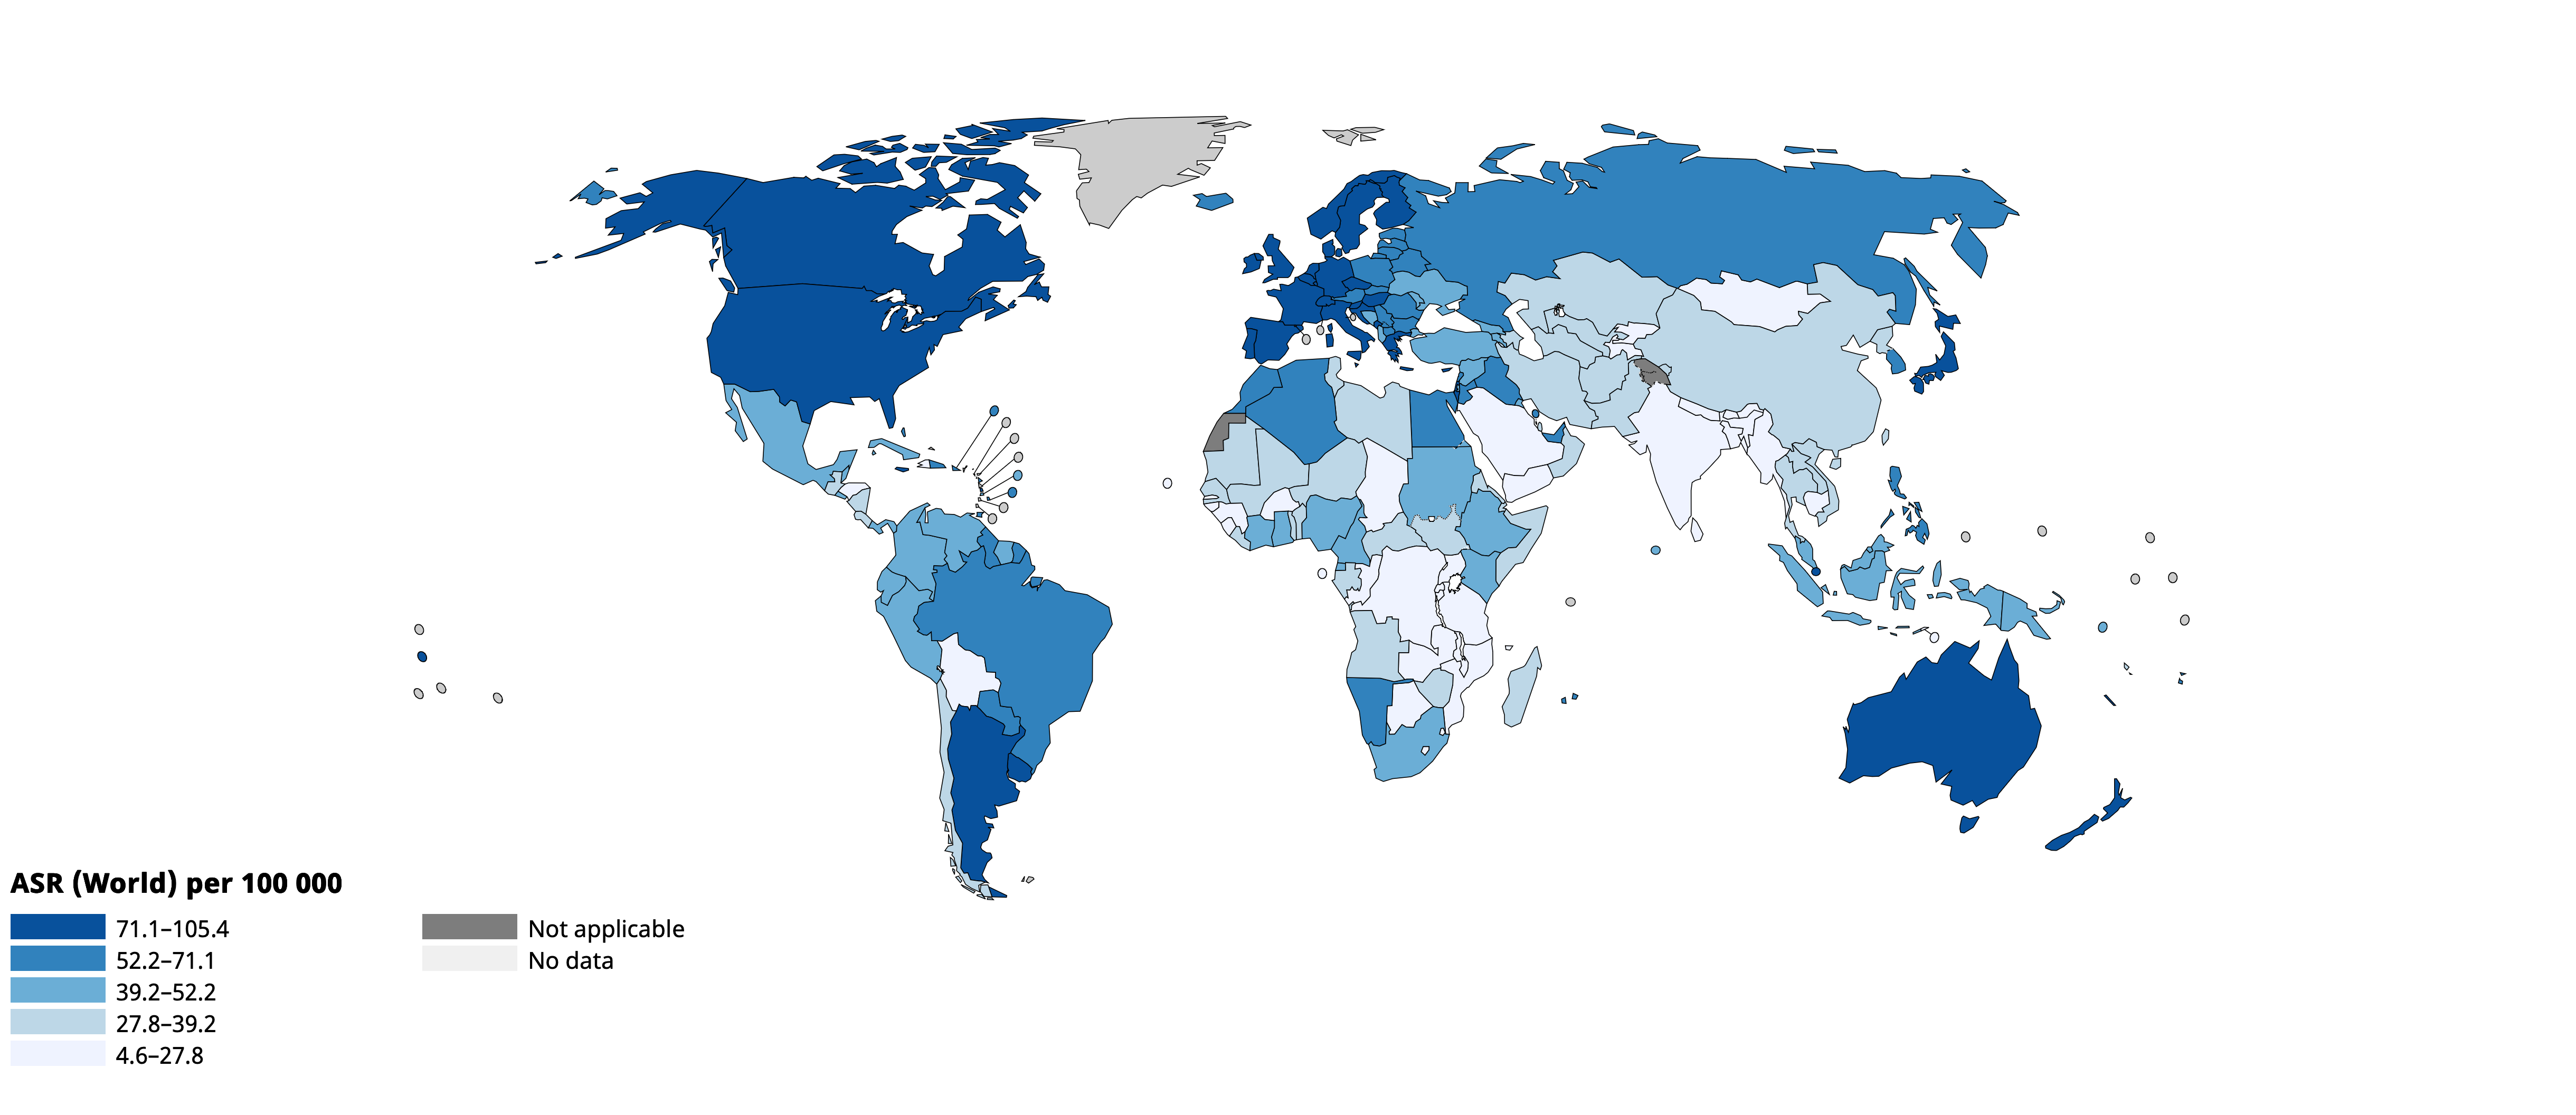
\includegraphics[width=1.0\textwidth]{/Users/JoseRomano/Documents/Tese/bca-thesis/Chapters/Figures/graphic_incidencies_world.png}
  \caption{Age-standardized incidence rate (ASR, per 100,000 inhabitants) of breast cancer in both sexes in 2022. The data represent global estimates based on \textcite{GLOBOCAN2022}, highlighting significant geographical variations in disease burden.}
\end{figure}

\begin{figure}[h!]
  \centering
  \begin{subfigure}[b]{0.8\textwidth}
    \centering
    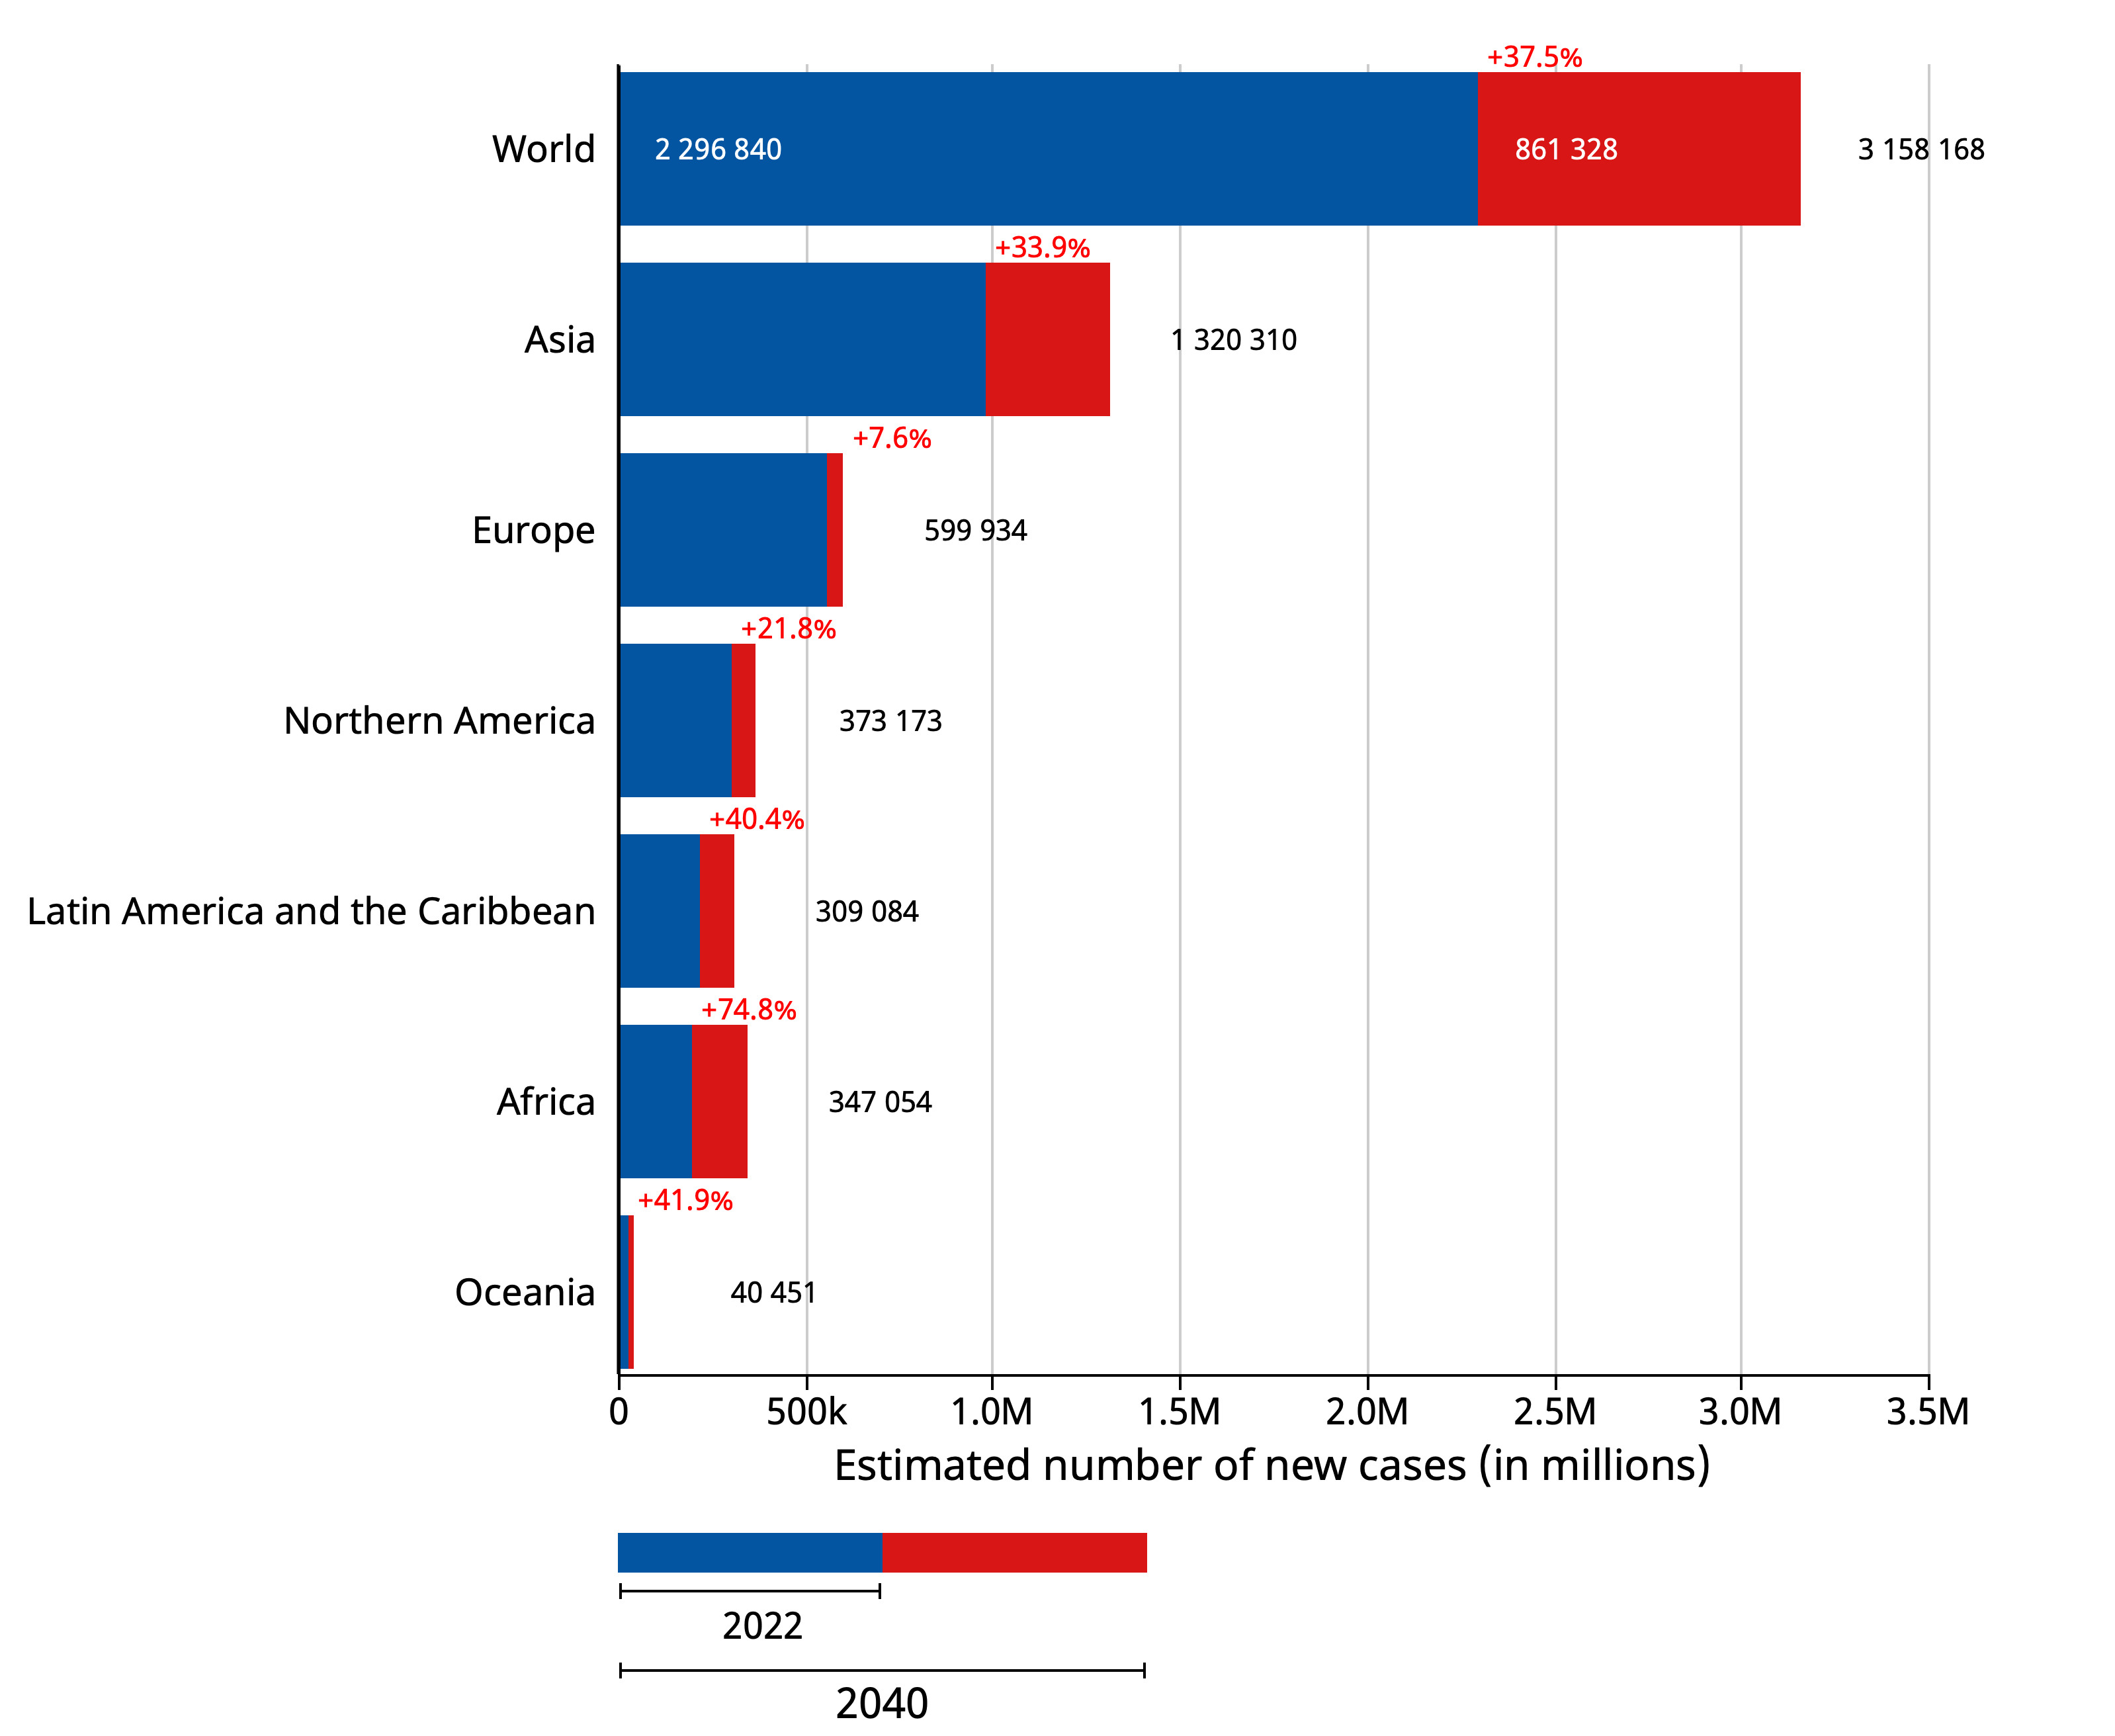
\includegraphics[width=\textwidth]{/Users/JoseRomano/Documents/Tese/bca-thesis/Chapters/Figures/new_cases_2020_2040.png}
    \caption{NEW CASES}
    \label{fig:imagem1}
  \end{subfigure}
  \vspace{0.5cm}
  \begin{subfigure}[b]{0.8\textwidth}
    \centering
    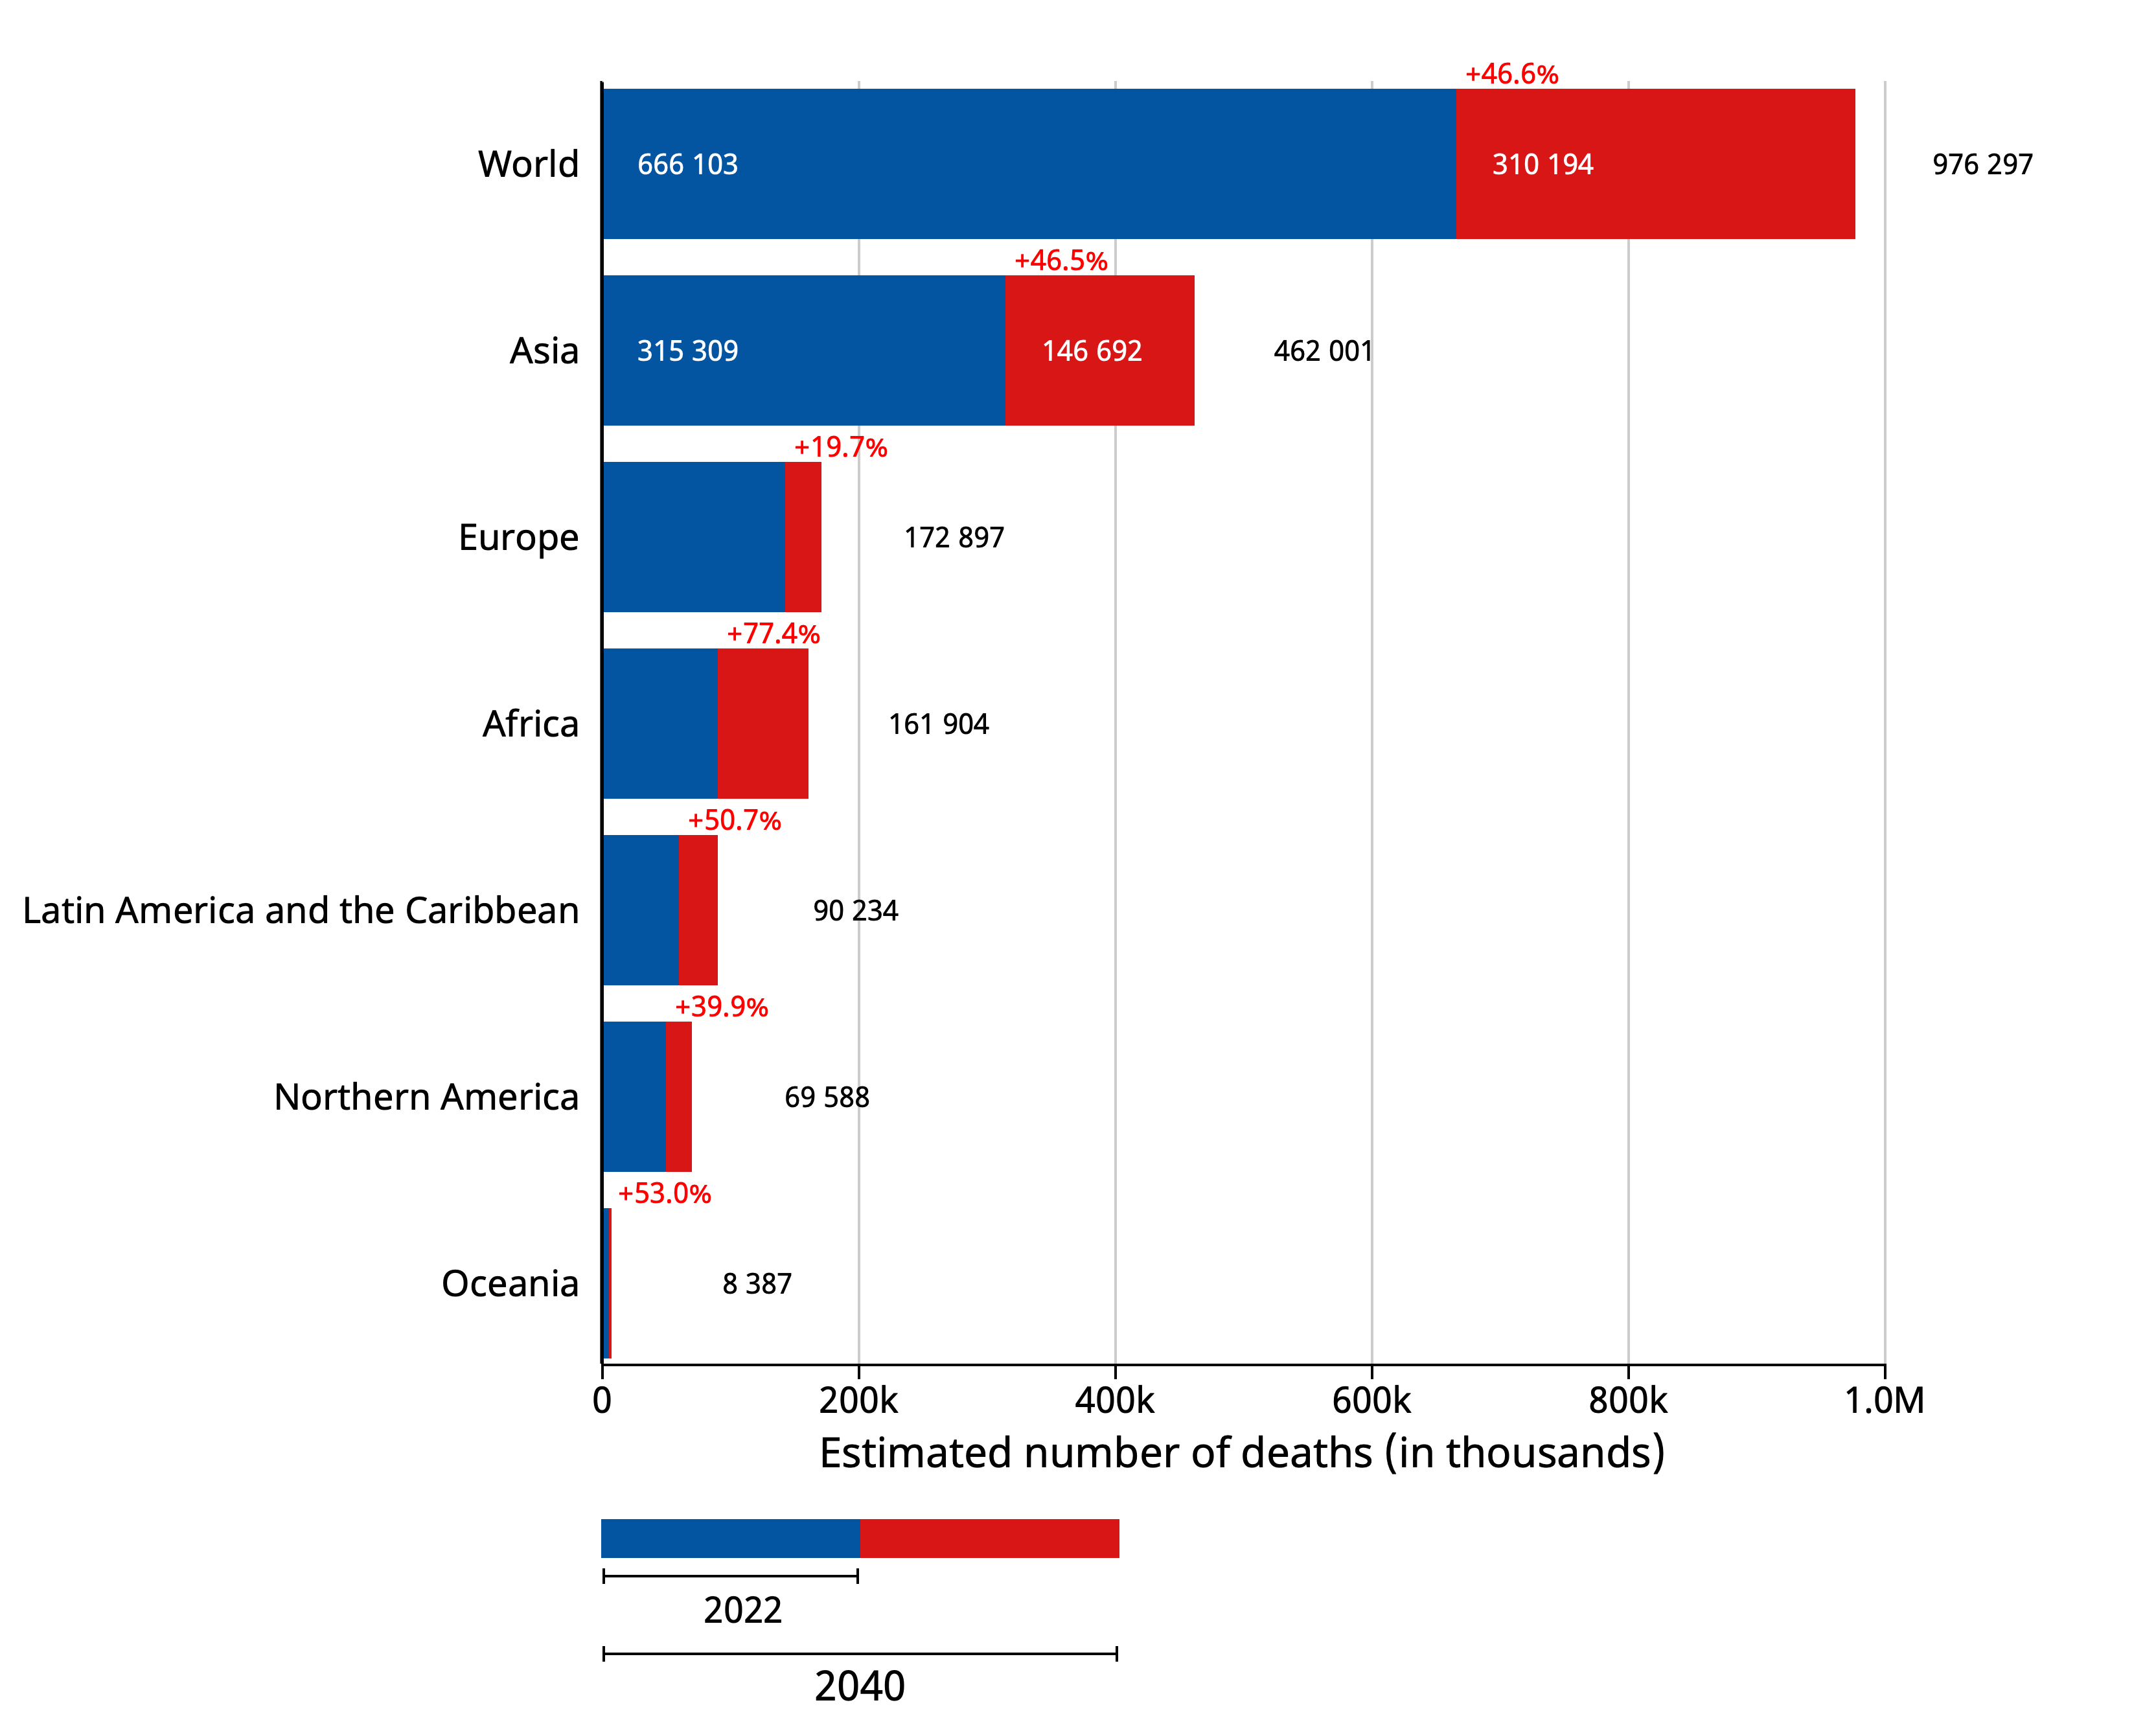
\includegraphics[width=\textwidth]{/Users/JoseRomano/Documents/Tese/bca-thesis/Chapters/Figures/deaths_2020_2040.png}
    \caption{MORTES}
    \label{fig:imagem2}
  \end{subfigure}
  \caption{Comparação visual entre dois cenários de interesse.}
  \label{fig:duas-imagens-empilhadas}
\end{figure}

BC is characterized by marked biological heterogeneity, manifested in multiple
molecular subtypes that exhibit distinct clinical behaviors
\textcite{bc_molecular_Perou2000}. Each subtype exhibits substantial
differences in terms of tumor aggressiveness, metastatic potential, and
behavior to specific therapies \textcite{bc_subtypes_Prat2015Clinical}. Thus,
accurate classification of these subtypes is essential to enable personalized
therapeutic approaches, with a direct impact on treatment efficacy and patient
prognosis \textcite{need_for_subtype_treatments_Testa2020Breast}.

\subsection{Can we improve the classification of Breast Cancer subtypes?}
Among the emerging candidates for robust biomarkers for the classification of
\gls{BC} subtypes are \gls{miRNAs}, small non-coding RNA molecules that play a
crucial regulatory role in gene expression. They are estimated to modulate the
expression of about one-third of the genes in the human genome
\textcite{mirna_importance_Hammond2015An} and are implicated in the regulation
of multiple physiological and pathological processes, including various human
diseases \textcite{mirna_as_biomarkers_Ho2022}.

Given their regulatory nature, several studies have demonstrated a significant
association between \gls{miRNAs} expression profiles and relevant clinical
characteristics in the context of \gls{BC}, including processes such as tumor
progression and metastasis development \textcite{mirna_as_biomarkers_Ho2022}
\textcite{mirnas_in_bc_Muñoz2023}
\textcite{mirna_as_bio_for_sub_Blenkiron2007MicroRNA}. In addition to these
aspects, a seminal study by Blenkiron \textit{et al.} (2007) demonstrated that
\gls{miRNAs} expression profiles can effectively distinguish between different
molecular subtypes of \gls{BC}, highlighting their potential as a precise
subtyping tool. This ability to discriminate between subtypes reinforces the
value of \gls{miRNAs} as promising clinical biomarkers.

\subsection{How to identify the most relevant miRNAs?}

The identification of the most relevant \gls{miRNAs} for \gls{BC} subtyping
represents a major analytical challenge due to the complexity of these high
dimensional regulatory molecules, non-linearity interactions between and
clinical phenotypes require advanced computational approaches to be effectively
modelled. Recent advances in \gls{AI}, particularly in \gls{ML} and \gls{DL},
have demonstrated remarkable potential in extracting meaningful patterns from
high-dimensional and heterogeneous (data from distinct nature) biomedical data.
These approaches enable not only the accurate classification of \gls{BC}
subtypes but also the identification of discriminative \gls{miRNAs} signatures,
supporting their integration as actionable biomarkers in clinical workflows.

In this context, \gls{ML} and \gls{DL} models are particularly well suited for
the task of robustly characterizing and explaining the profiles of
\gls{miRNAs}-based biomarkers — should such biomarkers exist — with the
potential to effectively discriminate between different \gls{BC} subtypes, as
already seen in a study done by \textcite{ml_gastric_Azari2023} Azari
\textit{et al.} 2023 where \gls{ML} algorithms identified potential diagnostic
and prognostic \glossary{miRNAs} in gastric cancer, showing high accuracy in
the identification of reliable biomarkers for this disease.

This reality reinforces the urgency of developing advanced computational tools
that can enable more precise molecular characterization and guide personalized
therapeutic decisions, ultimately improving clinical outcomes for patients with
aggressive and hard-to-treat \gls{BC} subtypes.

\section{Challenges and research hypothesis}
\label{sec:challenges+research-hypothesis}
Based on the assumption that it is possible to use microRNA expression values
and clinical data to map \glossary{BC} subtypes
(\textcites{mirna_as_biomarkers_Ho2022}{mirnas_in_bc_Muñoz2023}), this dissertation
proposes to explore several complementary directions for this pathology where
the application of \glossary{AI} techniques is still growing.

First, we intend to assess whether discriminative linear models perform better
than latent representation models (in a context where there are two different
data sources and many dimensions) - such as DIABLO \textcite{DIABLO_Singh2019},
a widely used model. At the same time, we will investigate the impact of
patient clinical information (such as age, presence or absence of metastases,
hormone levels, among others) on the classification performance of the models,
where we will be able to gain valuable insights into possible relationships
between these features and \glossary{BC} subtypes.

If substantial results are obtained by any of the models, we will be able to
conduct a more extensive study on our main point: whether or not there are
\gls{miRNAs} that are potential biomarkers for \glossary{BC} subtypes. In a
more advanced approach, I will be able to explore the applicability of
\textit{Conformal Prediction} \textcite{conformal_prediction_Angelopoulos2023},
which provides statistically based confidence intervals for each prediction
(which is widely used in areas where risk must be justified and well-founded,
such as finance and healthcare). The latter is an approach that is still
gaining ground in healthcare and, considering our problem, it makes sense to be
able to give a prediction based on a confidence interval, giving our model
greater transparency and reliability, something particularly relevant in
clinical contexts where error must be minimized and uncertainty well
characterized.

Even though the base seems promising, there are several challenges to overcome
in order to achieve the desired results such as:

\textbf{1. Biological heterogeneity:} \\
\label{sec:biological-heterogeneity}
Biological heterogeneity is characterized by the diversity of living organisms,
including species, genotypes, and populations, which exhibit a variety of
biological characteristics, such as morphology, physiology, genetics, and biogeography.
The human body is a highly complex system in which the behavior of each
component depends on its interaction with countless other parts.
Exposure to the same treatment by two bodies can result in completely different
reactions.

\textbf{2. Functional complexity of microRNAs:} \\
The role of \gls{miRNAs} in biological regulation and cancer progression is
extremely complex and still relatively new from a scientific point of view.
The action of a single microRNA is not isolated, but rather part of a network
of interactions with dozens (or hundreds) of other \gls{miRNAs} and contextual
factors. This highly interdependent behavior raises questions about the
effectiveness of overly simplistic or linear models. The application of
nonlinear models allows for the discovery of complex relationships and
cross-interactions between different \gls{miRNAs} or between them and clinical
variables. These relationships and interactions would be invisible to more
traditional approaches.

\textbf{3. No control set:} \\
Another relevant challenge is the absence of a control set that includes data
from healthy individuals. Since this type of analysis (\glossary{miRNA} expression
profiling) is not routinely performed in individuals without cancer, it is
difficult to define what would be a “normal level” of expression. The
implementation of a control group would not only broaden the scope of the
model's task (e.g., distinguishing between the presence and absence of cancer
before predicting the subtype), but also optimize the robustness of biomarker
identification. An illustrative example of this phenomenon is presented in the
study \textcite{ml_gastric_Azari2023} where the implementation of a control set
was fundamental to the identification of discriminative markers.

The data for this study were previously selected by Dr. Bárbara Mendes and her
team based on purely biological selection criteria. These criteria included the
scientific interest of the group and molecular characteristics that were
considered relevant in the context of the research ( CONFIRMAR NA REUNIÃO).
Consequently, the dataset I was given consists of 256 samples and 888
\glossary{miRNA} features, as well as 38 clinical data features. This presents
a scenario of high dimensionality with a limited number of examples on which to
train.

The morphology of this dataset limits the choice of approaches to be used and
requires extra caution in how we work with certain models, such as nonlinear
ones, given their high adaptability in high dimensions, which, in a context of
limited data, can easily lead to overfitting. This requires careful selection
of algorithms and attention to the pipeline that is set up to ensure that the
results obtained are robust and relevant.

Furthermore, this problem cannot be addressed with data augmentation techniques
used in the field of \glossary{ML}, such as \textit{SMOTE} (Synthetic Minority
Over-sampling Technique) \textcite{SMOTE_Blagus2013SMOTE}. As discussed earlier
in the topic \ref{sec:biological-heterogeneity}, the nature of this data makes
reliable synthetic generation unfeasible, which can lead to artificially
inconsistent samples ("Extra-terrestial beings", in other words).

Having a control set would be an important step toward increasing the
generalizability of our model. This data set would not only allow us to expand
the problem to include the distinction between healthy and sick individuals,
but also improve the identification of discriminative biomarkers. The latter
has already been successfully tested in other types of cancer, and a key step
in the pipeline used is precisely the comparison with a control set
(\textcite{ml_gastric_Azari2023}) to isolate clinically relevant markers.

\section{Document Organization}
\label{sec:document-organization}